\section{Methodology}
\label{sec:method}
\subsection{Description of the Proposed Project}

\subsubsection{Inputs}

All inputs are public and can be downloaded at the start of the project.
\begin{itemize}
  
  \item \textbf{Primary network and drug data: Hetionet~\cite{himmelstein2017hetionet}.}
  An integrated knowledge graph from which we use three edge types: protein--protein interactions (these include the interactome of Menche et al.~\cite{menche2015uncovering}), DrugBank-derived drug--target links, and disease--gene links for Alzheimer's disease. The processed network has $N=15{,}139$ proteins and $E=147{,}149$ edges, with 1{,}383 drugs that have at least one target in the network and 185 AD genes. Edges are unweighted and undirected. Hetionet combines sources with mixed licenses, some non-commercial, so we do not redistribute raw data  as illustrated in \ref{fig:example of a network module}).
\begin{figure}[h]
    \centering
    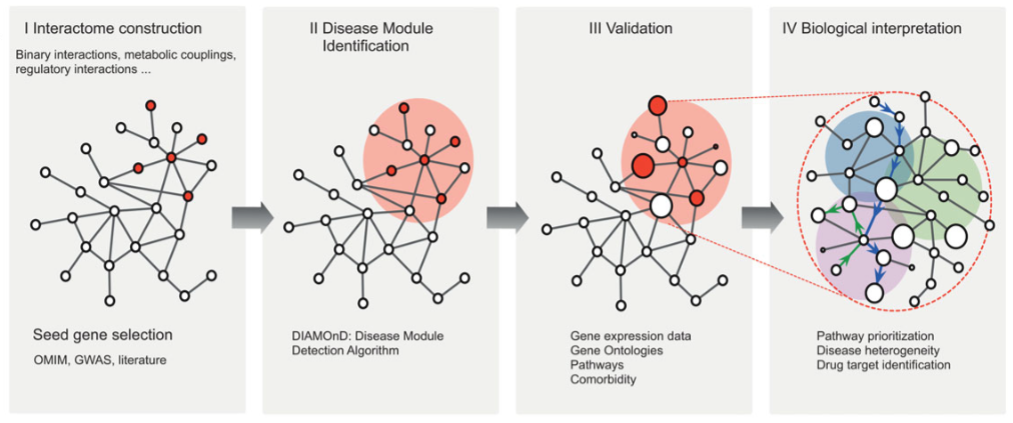
\includegraphics[width=0.5\linewidth]{images/network_module.png}
    \caption{Example of identifying a network module}
    \label{fig:example of a network module}
\end{figure}
  
  \item \textbf{Comparison network: BioGRID~\cite{oughtred2021biogrid}.} Human physical interactions: $N=17{,}602$ and $E=679{,}846$ (about 4.6 times as many edges), with 1{,}382 drugs and 191 AD genes mapped. It is the heavier workload for the timing experiments. STRING~\cite{szklarczyk2023string} at several confidence cut-offs is an optional further comparison, and  ChEMBL~\cite{zdrazil2024chembl} or DGIdb~\cite{freshour2021dgidb} drug--target data can replace the DrugBank-derived links as a robustness check as illustrated in  \ref{fig:disease-module}).
\begin{figure}[h]
    \centering
    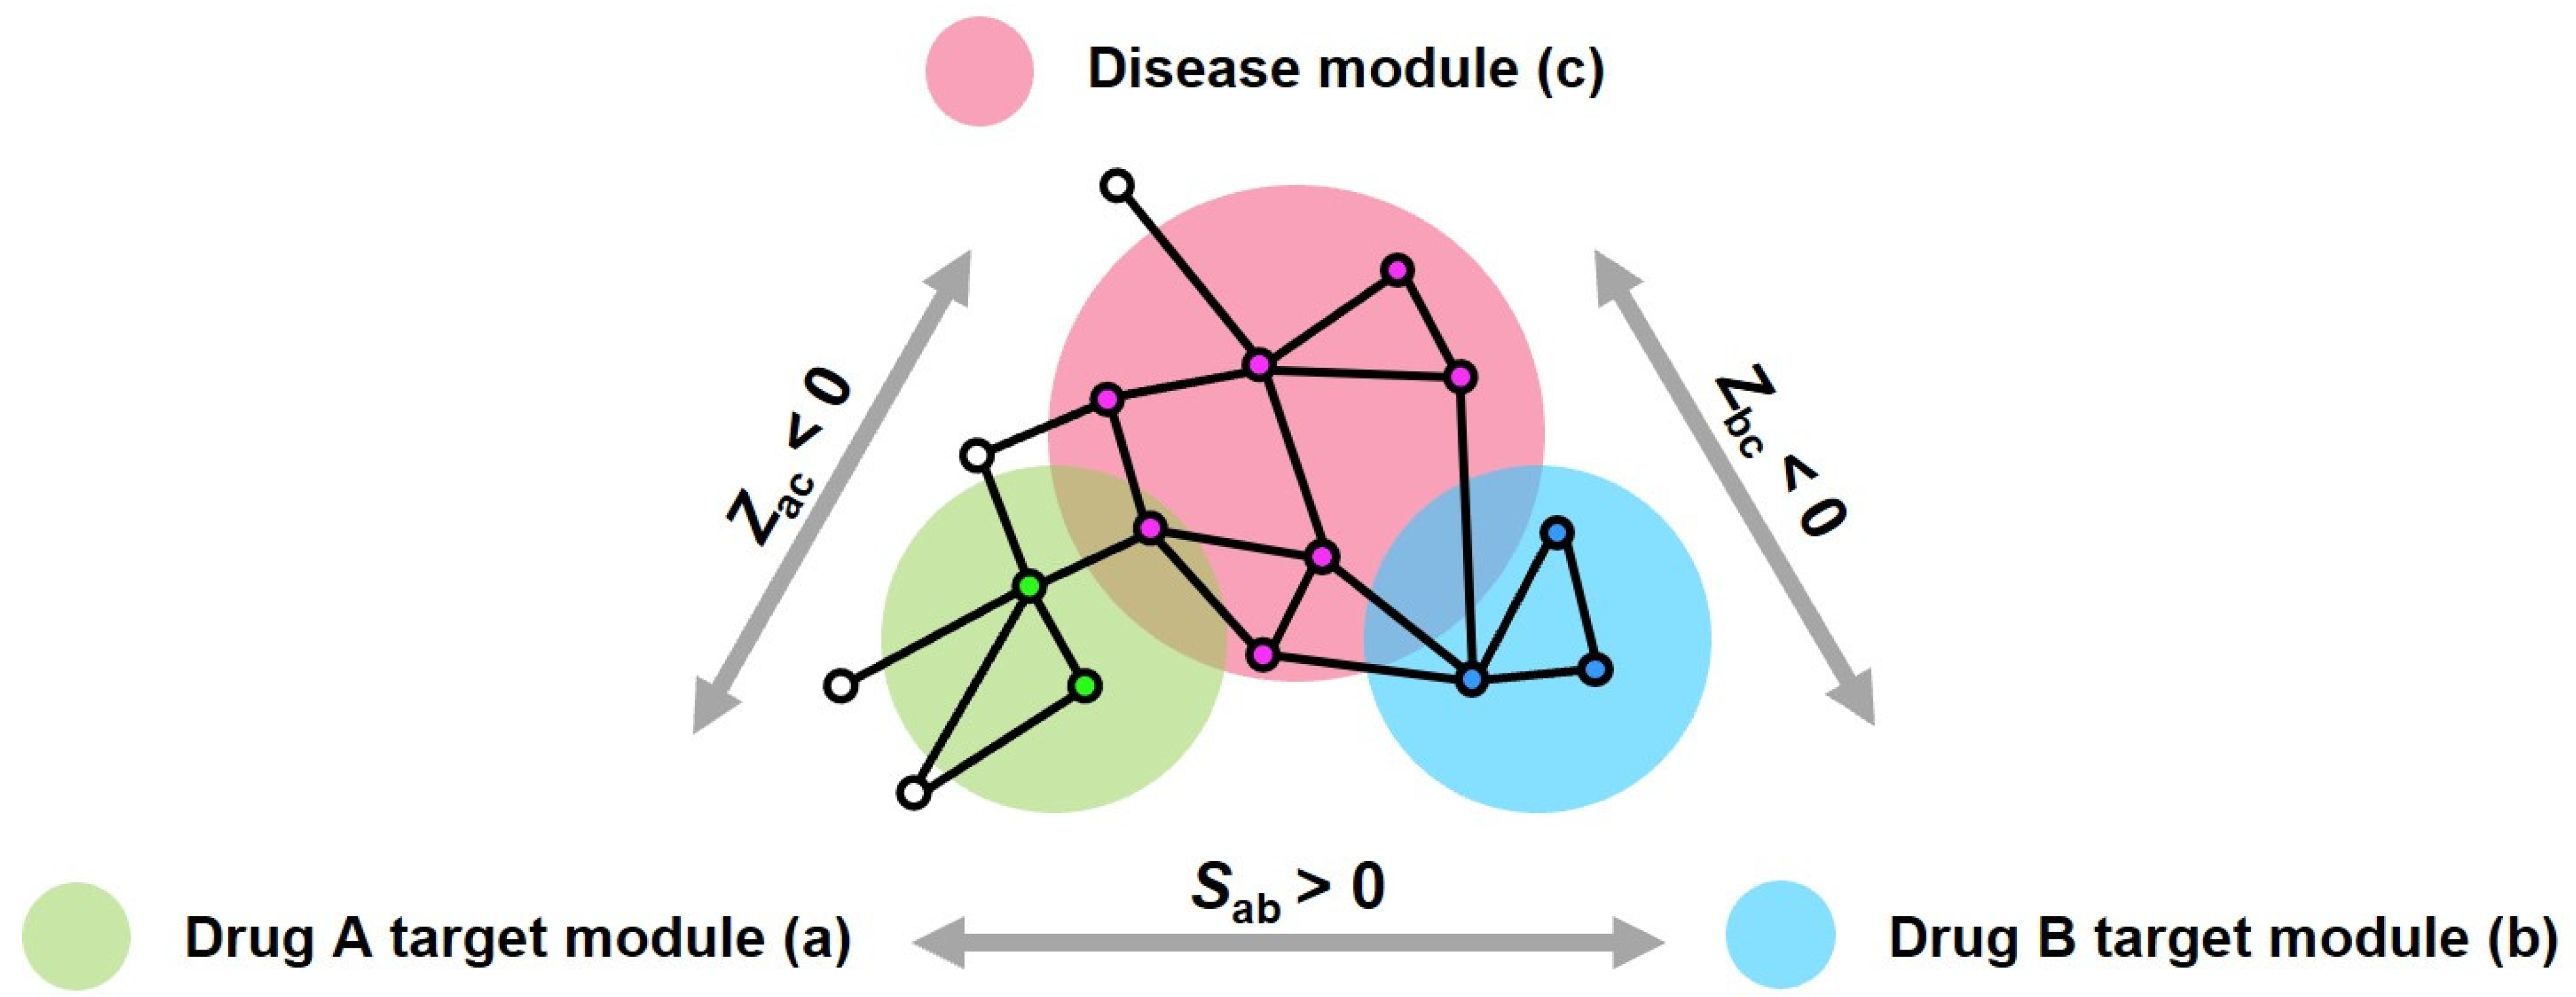
\includegraphics[width=0.5\linewidth]{images/network_drug.png}
    \caption{Example of a drug targeting a disease module}
    \label{fig:disease-module}
\end{figure}
  
  \item \textbf{AD disease module.} Hetionet's disease--gene links for Alzheimer's disease (185 proteins). An alternative module built from the largest recent genetic study~\cite{bellenguez2022new} plus well-known AD genes (e.g., \textit{APP}, \textit{PSEN1}, \textit{PSEN2}, \textit{APOE}, \textit{MAPT}) is a robustness variant.
  
  \item \textbf{Validation list.} About 30 drugs that have entered AD clinical trials. The list was compiled from general knowledge and \textbf{must be verified} against ClinicalTrials.gov and the annual AD drug-development pipeline review~\cite{cummings2024pipeline} before any result is reported. 
  
  \item \textbf{Parameters.} Number of random samples per drug $R\in\{100, 1{,}000, 10{,}000\}$, and, for the optional part, shortlist size $n\le 28$ and combination size $k$.
\end{itemize}

The GPU only ever sees three things: a graph (who connects to whom), a few
thousand small lists of node IDs (each drug's targets), and one more list of
node IDs (the AD module). Everything biological is just labels on those
node IDs.

\subsubsection{Proposed Process}

The screen answers one question for every drug: \emph{are this drug's targets
closer to the AD module than we would expect by chance?}

\begin{enumerate}
  \item \textbf{Distance.} For each target of the drug, find the shortest
        path (fewest edges) to the nearest AD protein, and average these over
        the drug's targets. This is the drug's \emph{proximity} $d$; smaller
        means closer.
  \item \textbf{Chance level.} Repeat the same calculation $R$ times using
        random ``fake'' target sets and random ``fake'' AD modules of the same
        sizes, where each random protein is picked to have a similar number
        of connections as the real one it replaces. This gives the average
        $\mu$ and spread $\sigma$ of proximity by chance.
  \item \textbf{Score.} $z = (d-\mu)/\sigma$. A strongly negative $z$ (for
        example $z < -2$) means the drug is unusually close to AD.
\end{enumerate}

\paragraph{(i) Processes parallelized with SIMT (GPU/CUDA).}
\begin{enumerate}
  \item \textbf{All-pairs shortest-path distances.} One BFS from every node gives the full distance matrix $D$, where $D[a][b]$ is the number of steps from protein $a$ to protein $b$. Since distances in this network are small (rarely above 15), each entry fits in one byte. We run many BFS searches at once using \emph{bit-parallel multi-source BFS}~\cite{then2014more}: each node keeps one bit per search, so a 64-bit word tracks 64 searches, and one step of all 64 searches becomes a bitwise OR over the node's neighbors.
  \item \textbf{Proximity and random sampling .} Every (drug, random sample) pair is independent. Each GPU thread generates one random sample, looks up the needed distances in $D$, takes minimums and an average, and a block-level reduction combines the samples into $\mu$ and $\sigma$ for that drug.
  % \item \textbf{Drug--drug separation } For the shortlist, the distance-based separation between every pair of drugs, computed with the same look-up-and-minimum pattern.
  % \item \textbf{Exact QUBO solver (Module 5, optional).} Tries all $2^n$ yes/no choices for $n$ shortlisted drugs, one GPU thread per group of choices; practical up to $n\approx 30$.
  % \item \textbf{QAOA simulation (Module 5, optional).} Simulated with cuQuantum's cuStateVec, which itself runs data-parallel over the $2^n$ numbers that describe the quantum state.
\end{enumerate}

\paragraph{(ii) Related works and how this implementation differs.}
Network proximity for drug repurposing was introduced by Guney et al.~\cite{guney2016network} and has been applied to AD several times~\cite{fang2021endophenotype,csbj2023proximity,lqt2025proximity}. These studies focus on the biology and generally run the screen as sequential scripts. GPU BFS is well studied~\cite{harish2007accelerating,merrill2012scalable,wang2016gunrock}, and bit-parallel MS-BFS was designed for running many searches over one graph~\cite{then2014more}, but these are general-purpose graph tools, not proximity screens. 
% Quantum drug-combination selection was recently formulated as a QUBO and solved with quantum annealing~\cite{qmi2026combinations}.

Our implementation differs in that it:
\begin{itemize}[nosep]
  \item runs the \emph{whole} screen on the GPU, including the random sampling, which is usually the slowest part;
  \item stores distances as one byte each and produces them with bitwise MS-BFS, so the full matrix for 20{,}000 proteins (400~MB) stays on the GPU and every later step is a fast memory look-up;
  \item uses the same counter-based random number generator on CPU and GPU, so both versions draw identical random samples and their results can be compared exactly;
  \item targets AD specifically and checks results against AD trial drugs;
  % \item (Optional) benchmarks simulated gate-based QAOA against the exact optimum and classical solvers on the same biology-derived instances, instead of reporting a quantum solution alone.
\end{itemize}

\paragraph{(iii) Parallelization plan.}
\begin{center}
\small
\begin{tabularx}{\linewidth}{@{}lXl@{}}
\toprule
Step & How work is split across GPU threads & Limited by \\
\midrule
Multi-source BFS & Sources processed in batches of $64\times W$ (e.g., 1{,}024). One thread per (node, 64-bit word). Each level: OR the neighbors' frontier words, AND with NOT-visited, write the level number into $D$ for newly reached sources. Graph stored in CSR form. Repeat until no bits change. & Memory \\
Writing $D$ & Threads for neighboring nodes write neighboring bytes of the same row of $D$, so writes are coalesced. & Memory \\
Proximity + $z$-score & One thread block per drug; each thread handles several random samples; degree-matched sampling from per-degree-bin node lists; distances read from $D$ (reads are scattered, so L2 cache matters); block reduction for $\mu$, $\sigma$. & Memory \\
Drug--drug separation & One thread per drug pair on the shortlist; same look-up pattern. & Memory \\
% QUBO brute force & One thread per block of $2^{m}$ bit patterns; patterns visited in Gray-code order so each step flips one bit and updates the cost in $O(n)$; warp and block minimum reduction. & Compute \\
\bottomrule
\end{tabularx}
\end{center}
Data moves to the GPU once (the graph and ID lists, a few MB) and results come back once ($z$-scores; $D$ only if needed).

\paragraph{(iv) Processes not parallelized.}
\begin{itemize}[nosep]
  \item Downloading and reading the databases; converting between gene and protein identifiers; removing duplicates and self-loops.
  \item Building the CSR graph and keeping its largest connected component.
  \item Grouping proteins into degree bins for the random sampling.
  \item Ranking drugs, computing validation metrics, and plotting.
  % \item Building the QUBO matrix from the separation results, and the classical optimizer loop that tunes QAOA's parameters.
\end{itemize}

\subsubsection{Outputs}

\begin{enumerate}
  \item \textbf{Distance matrix} $D$ for the interactome (binary file, one byte per entry), plus summary statistics (e.g., distance histogram).
  \item \textbf{Ranked drug list} with proximity $d$, $z$-score, and $p$-value for every drug, and the top AD repurposing candidates.
  \item \textbf{Execution-time comparison}: sequential C++ vs.\ CUDA time for (a) all-pairs distances and (b) proximity scoring, across network sizes $N$ and random-sample counts $R$, with speedup charts.
  \item \textbf{Correctness report}: GPU and CPU distance matrices are identical, and $z$-scores match when using the same random samples.
  \item \textbf{Validation}: how highly AD trial drugs are ranked, compared with simple baselines.
  % \item \textbf{(Optional) Combination results}: best $k$-drug combinations from the shortlist, and each solver's solution quality (including simulated QAOA) compared with the exact answer.
\end{enumerate}

%======================================================================
\section{Proposed Target Implementation Platform}
\label{sec:platform}

\begin{center}
\small
\begin{tabularx}{\linewidth}{@{}lX@{}}
\toprule
Component & Specification \\
\midrule
Parallel paradigm & SIMT on NVIDIA GPUs via CUDA C++ (primary); AVX2 SIMD on the CPU as a baseline; hand-written AVX-512/assembly only as an optional extra \\
GPU & NVIDIA GeForce GTX 1660: Turing (TU116), compute capability 7.5, 1{,}408 CUDA cores, 6 GB GDDR5 on a 192-bit bus, 192 GB/s \cite{gtx1660_specs}. GeForce cards are slow at 64-bit floating point, so all GPU code uses 32-bit integers (deterministic mode) or 32-bit floats. \\
CPU (baselines) & Processor	AMD Ryzen 5 3500 6-Core Processor, 3600 Mhz, 6 Core(s), 6 Logical Processor(s); Cache: L1 cache: 384KB, L2 cache: 3.0 MB, L3: 16.0 MB; RAM: 16GB. Must support AVX2 and FMA; AVX-512 is not assumed. Same machine as the GPU. \\
OS & Linux (Ubuntu 22.04/24.04), or Windows with WSL2 \\
GPU libraries & CUDA Toolkit 12.x, CUB (block reductions), a counter-based RNG (Philox, as in cuRAND/Random123) shared with the CPU code\\ % cuQuantum (cuStateVec) through CUDA-Q for the optional part \\
Languages and build & C++17 and CMake for the core; Python 3.11+ (pandas, NumPy, SciPy, matplotlib) for data preparation, validation, and plots; NetworkX as an independent reference on small graphs \\
Profiling & Nsight Systems and Nsight Compute \\
Repository & GitHub: source, build and benchmark scripts, the discussion of the parallel algorithms, and the sequential-vs-parallel timing results required for Milestone~3 \\
\bottomrule
\end{tabularx}
\end{center}

%======================================================================
\section{Mid-Project Milestones}
\label{sec:milestones}

\paragraph{Milestone 2 (Week 10) deliverable.} A live demo on the Hetionet
interactome that shows:
\begin{enumerate}[nosep]
  \item the GPU multi-source BFS producing the full distance matrix, and a check that it is identical to the sequential C++ result;
  \item the GPU proximity and $z$-score step for all drugs with $R=1{,}000$ random samples;
  \item a first sequential-vs-parallel timing table for both steps;
  \item a first ranked list of AD candidates.
\end{enumerate}

The full schedule is in Table~\ref{tab:schedule}.

\begin{table}[h]
\centering
\small
\begin{tabularx}{\linewidth}{@{}lX@{}}
\toprule
Week & Work \\
\midrule
6 & Proposal submission (Milestone 1). Download and freeze data versions. Set up repository and CMake build. \\
7 & Data preparation (identifier mapping, CSR graph, degree bins). Sequential C++ BFS and proximity; check against NetworkX on a small graph. \\
8 & GPU multi-source BFS; exact comparison with the CPU distance matrix. \\
9 & GPU proximity and $z$-score kernel with shared RNG; timing harness (CUDA events, median of 10 runs). \\
10 & \textbf{Milestone 2: mid-project demo} (above). \\
11 & Scaling experiments (Hetionet vs.\ BioGRID, optionally STRING cut-offs; $R$ up to 10{,}000); profiling; validation against AD trial drugs and baselines. \\
% 12 & (Optional) Drug--drug separation, QUBO, GPU brute force, classical heuristics, and simulated QAOA via CUDA-Q (benchmark, Appendix). \\
13 & \textbf{Milestone 3}: final GitHub submission with source, parallel-algorithm discussion, and sequential-vs-parallel timing; demo; optional conference paper. \\
\bottomrule
\end{tabularx}
\caption{Project schedule by academic week.}
\label{tab:schedule}
\end{table}
